\documentclass{beamer}


\usepackage{pgfpages}
%\setbeameroption{show notes}
%\setbeameroption{show notes on second screen=right}
\mode<presentation> {
  \usetheme{Warsaw}
  % ou autre ...

  \setbeamercovered{transparent}
  % ou autre chose (il est également possible de supprimer cette ligne)
}


\usepackage[french]{babel}
\usepackage[latin1]{inputenc}
\usepackage{times}
\usepackage[T1]{fontenc}
\usepackage{tikz}
\pgfdeclareimage[height=0.5cm]{le-logo}{logo-irisa}
\logo{\pgfuseimage{le-logo}}
\setbeamertemplate{footline}[frame number]


%%%%%%%%%%%%%%%%%%%%%%%%%%%
\title[Patterns for SoS Reconfiguration] 
{Approach Based Patterns for System-of-Systems Reconfiguration}
%\subtitle {ne compléter que si l'article possède un sous-titre}

\author[Franck, Petitdemange] 
{F.~Petitdemange\inst{1} \and I.~Borne\inst{1} \and J.~Buisson\inst{2}}

\institute[]
{
  \inst{1}%
  IRISA\\
  University of South Brittany\\
  Vannes, France
  \and
  \inst{2}%
  IRISA\\
  Military Academy of St-Cyr\\
  Vannes, France}

\date[SESOS 2015] 
{Software Engineering for Systems-of-Systems, 2015}



\begin{document}


\begin{frame}
  \titlepage
\end{frame}

\begin{frame}{Plan}
  \tableofcontents
\end{frame}

\section{Introduction}

\subsection{SoS Engineering Process}
\begin{frame}{SoS Engineering Process}
  %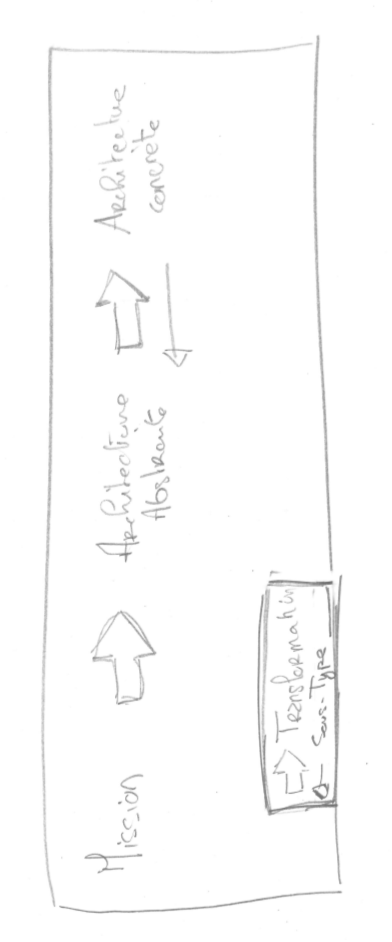
\includegraphics[scale=0.3, angle=-90]{construction-process}
  \begin{tikzpicture}
  \tikzstyle{format} = [draw, thin]
  %\draw (0,0) rectangle (1,1) node [pos=0.5] {Mission};
  %\draw (0,0) rectangle (1,1) node [pos=0.5] {Abstract Architecture};
  \draw (0,0) node[format] (mis) {Mission};
  \draw (3,0) node[format] (ab) {Abstract Arch.}; 
  \draw [->] (mis) edge (ab);
  \draw (7,0) node[format] (ca) {Concrete Arch.};
  \draw [->] (ab) edge (ca);

\draw (0,-1) node [draw, thin] (leg) {raffined };
\end{tikzpicture}
\end{frame}

\subsection{SoSADL}
\begin{frame}{Architecture desciption language : SoSADL}
\begin{description}
  \item[Constituent System (CS) :] have their own managerial and
    operational independance while contributing to the global mission
    of the SoS
  \item[Mediator :] controled by the SoS. They belong to the
    SoS. Mediateur are communicating element that specify, coordinate
    the interaction beetween CSs and SoS control over them.
  \item[Coalition :] a set of contraints about the CSs and
    mediator required to accomplish a emergent behavior.
\end{description}
\end{frame}

\subsection{Context}
\begin{frame}{Emergency service SoS}
\begin{description}
  \item[Mission :] preserve human life and material
\end{description}
\newcommand{\labelSystem}{system}
  \newcommand{\labelMediator}{mediator}
  \newcommand{\labelCoalition}{coalition}
  \newlength{\boxWidth}
  \settowidth{\boxWidth}{\labelSystem}
  \newlength{\tmp}
  \settowidth{\tmp}{1..n}
  \addtolength{\boxWidth}{\tmp}
  \addtolength{\boxWidth}{2.75em}
  \newcommand{\msbox}[7]{
    \node[minimum width=#6,minimum height=#7,draw] (#1) at (#2) {#3};
    \node[below right,font=\footnotesize,gray] (tmp) at (#1.north west) {#5};
    \draw (tmp.south west) -- (tmp.south east) -- ([xshift=1ex]tmp.north east);
    \node[below left,font=\footnotesize,gray] at (#1.north east) {#4};
  }
  \newcommand{\system}[4]{\msbox{#1}{#2}{#3}{#4}{\labelSystem}{\boxWidth}{4em}}
  \newcommand{\mediator}[4]{\msbox{#1}{#2}{#3}{#4}{\labelMediator}{\boxWidth}{2.5em}}
  \newcommand{\port}[2]{\node[fill=white,draw] (#1) at (#2) {};}
  \newcommand{\relation}[4]{
    \draw (#2) -- (#3);
    \node[above right,font=\footnotesize,gray] at (#2) {#1};
    \node[above left,font=\footnotesize,gray] at (#3) {#4};
  }
  \newcommand{\coalition}[2]{
    \node[draw,fit=#2,inner sep=1em,dashed] (#1) {};
    \node[below right,font=\footnotesize,gray] (tmp) at (#1.north west) {\labelCoalition};
    \draw[dashed] (tmp.south west) -- (tmp.south east) -- ([xshift=1ex]tmp.north east);
  }
\newcommand{\added}[1]{#1}



\clubpenalty = 10000
\widowpenalty = 10000
\displaywidowpenalty = 10000


    
\end{frame}

\section{Patterns for SoS reconfiguration}
\subsection{Motivation}
\begin{frame}{Need of architectural reconfiguration} 
  Cause :
  \begin{itemize}
  \item managerial and operational independance of the constituents
  \end{itemize}
  Consequence :
  \begin{itemize}
  \item architecture evolve continuesly
  \end{itemize}
  Problems :
  \begin{itemize}
  \item determine a set of reconfiguration' operations to maintain architectural pattern in the concrete architecture?
  \item determine a set of reconfiguration' operations to make evolve the architectural pattern in a coherently way?   
  \end{itemize}
\end{frame}

\begin{frame}{Architectural pattern}
  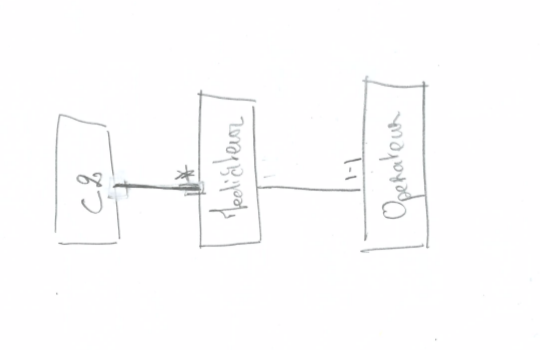
\includegraphics[angle=-90, scale=0.5]{pattern-emergency-service}
\end{frame}

\begin{frame}{Maintain architectural patterns}
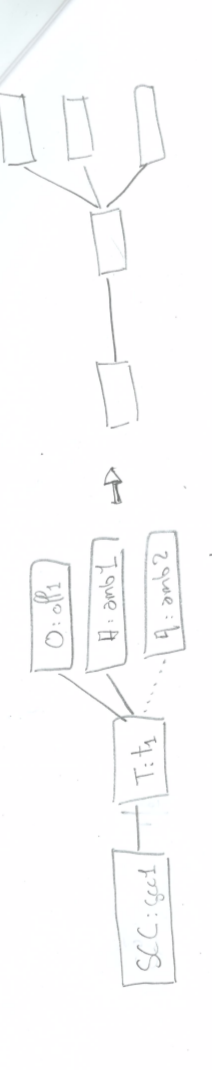
\includegraphics[angle=-90, scale=0.4]{cas-maintain-pattern}
\end{frame}

\begin{frame}{Architectural pattern evolutions}
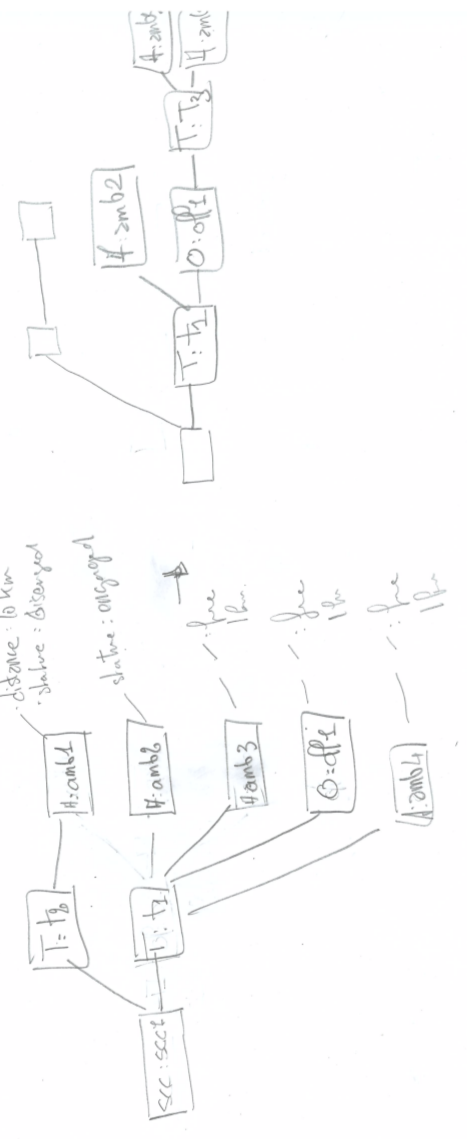
\includegraphics[angle=-90,scale=0.4]{cas-evolution-pattern}
\end{frame}

\subsection{Approach}
\begin{frame}{Patterns for reconfiguration}
  Approach :
  \begin{itemize}
  \item use pattern approach to formalize a set of best practice to assist
    reconfiguration
  \end{itemize}

  \begin{itemize}
  \item based on dedicaded language (SoSADL), describe SoS architecture
    pattern architectural taking into account SoS characteristics
  \item express a set of reconfiguration operations associate to this
    architectural pattern which can express for instance :when, how,
    for which to add a new CS.
  \end{itemize}
\end{frame}


\begin{frame}{Challenges}
  \begin{itemize}
  \item the choice of reconfiguration' operations in order to instanciate or reinstanciate the architectural pattern
  %\item ... 
  \end{itemize}
\end{frame}


\section{Related Works}

\begin{frame}{}
\end{frame}

\section{Conclusion}

\begin{frame}{Challenge and Futur Work}
  Challenge : 
  \begin{itemize}
  \item
  \end{itemize}

  Futur Work :
  \begin{itemize}
  \item
  \end{itemize}
\end{frame}

\end{document}